\documentclass[problem]{mcs}

\begin{pcomments}
  \pcomment{CP_coin_flip_sequences}
  \pcomment{second part of PS_coin_flip_sequences}
\end{pcomments}

\pkeywords{
  probability
  conditional_probability
  coin
  transitive
  intransitive
}

%%%%%%%%%%%%%%%%%%%%%%%%%%%%%%%%%%%%%%%%%%%%%%%%%%%%%%%%%%%%%%%%%%%%%
% Problem starts here
%%%%%%%%%%%%%%%%%%%%%%%%%%%%%%%%%%%%%%%%%%%%%%%%%%%%%%%%%%%%%%%%%%%%%

\begin{problem}
Suppose you repeatedly flip a fair coin until you see the sequence
\STR{HTT} or \STR{HHT}.  What is the probability you see the
sequence \STR{HTT} first?

\hint Try to find the probability that \STR{HHT} comes before
\STR{HTT} conditioning on whether you first toss an \STR{H} or a
\STR{T}.  The answer is not $1/2$.

\begin{solution}
Let $A$ be the event that \STR{HTT} appears before \STR{HHT}, and let
$p \eqdef \prob{A}$.

\iffalse Let $\pr{A}$ be the of seeing \STR{HTT} before \STR{HHT} if
you start at $A$, and define $pr{B}$ and $pr{C}$ similarly.  We are
trying to find $pr{A}$.

%, that is, the probability of seeing \STR{HTT} before \STR{HTT} if
%you start with no prior information.

Then,
\begin{align*}
Pr[A] &  = \frac12 Pr[A] + \frac12 Pr[B]\\
Pr[B] & = \frac14 + \frac14 Pr[B] + \frac14 Pr[C]\\
Pr[C] & = \frac12 Pr[C]
\end{align*}
Solving these equations (starting from the bottom going up), we get
\begin{align*}
            Pr[C] & = 0\\
Pr[B] - 1/4 Pr[B] & = 1/4 + 0\\
            Pr[B] & = 1/3\\
Pr[A] - 1/2 Pr[A] & = 1/2 * 1/3\\
            Pr[A] & = 1/3.
\end{align*}
So \STR{HTT} comes before \STR{HHT} with probability 1/3.
\fi

Suppose our first toss is \STR{T}.  Since neither of our patterns
starts with \STR{T}, the probability that $A$ will occur from this
point on is still $p$.  That is, $\prcond{A}{\tails} = p$.

Suppose our first toss is \STR{H}.  To find the probability that $A$
will now occur, that is, to find $r \eqdef \prcond{A}{\heads}$, we
consider different cases based on the subsequent throws.

Suppose the next toss is \STR{H}, that is, the first two tosses are
\STR{HH}.  Then neither pattern appears if we continue flipping
\STR{H}, and when we eventually toss a \STR{T}, the pattern
\STR{HHT} will then have appeared first.  So in this case, event $A$
will never occur.  That is $\prcond{A}{\mathtt{HH}} = 0$.

Suppose the first two tosses are \STR{HT}.  If we toss a \STR{T}
again, then we have tossed \STR{HTT}, so event $A$ has occurred.
If we next toss an \STR{H}, then we have tossed \STR{HTH}.  But this
puts us in the same situation we were in after rolling an \STR{H} on
the first toss.  That is, $\prcond{A}{\mathtt{HTH}} = r$.

This reasoning is illustrated in Figure~\ref{HTTHHT} which shows the
tree for the probability space underlying these events.  Although the
tree is infinite, it has a simple repeating structure.

\begin{figure}[h]
  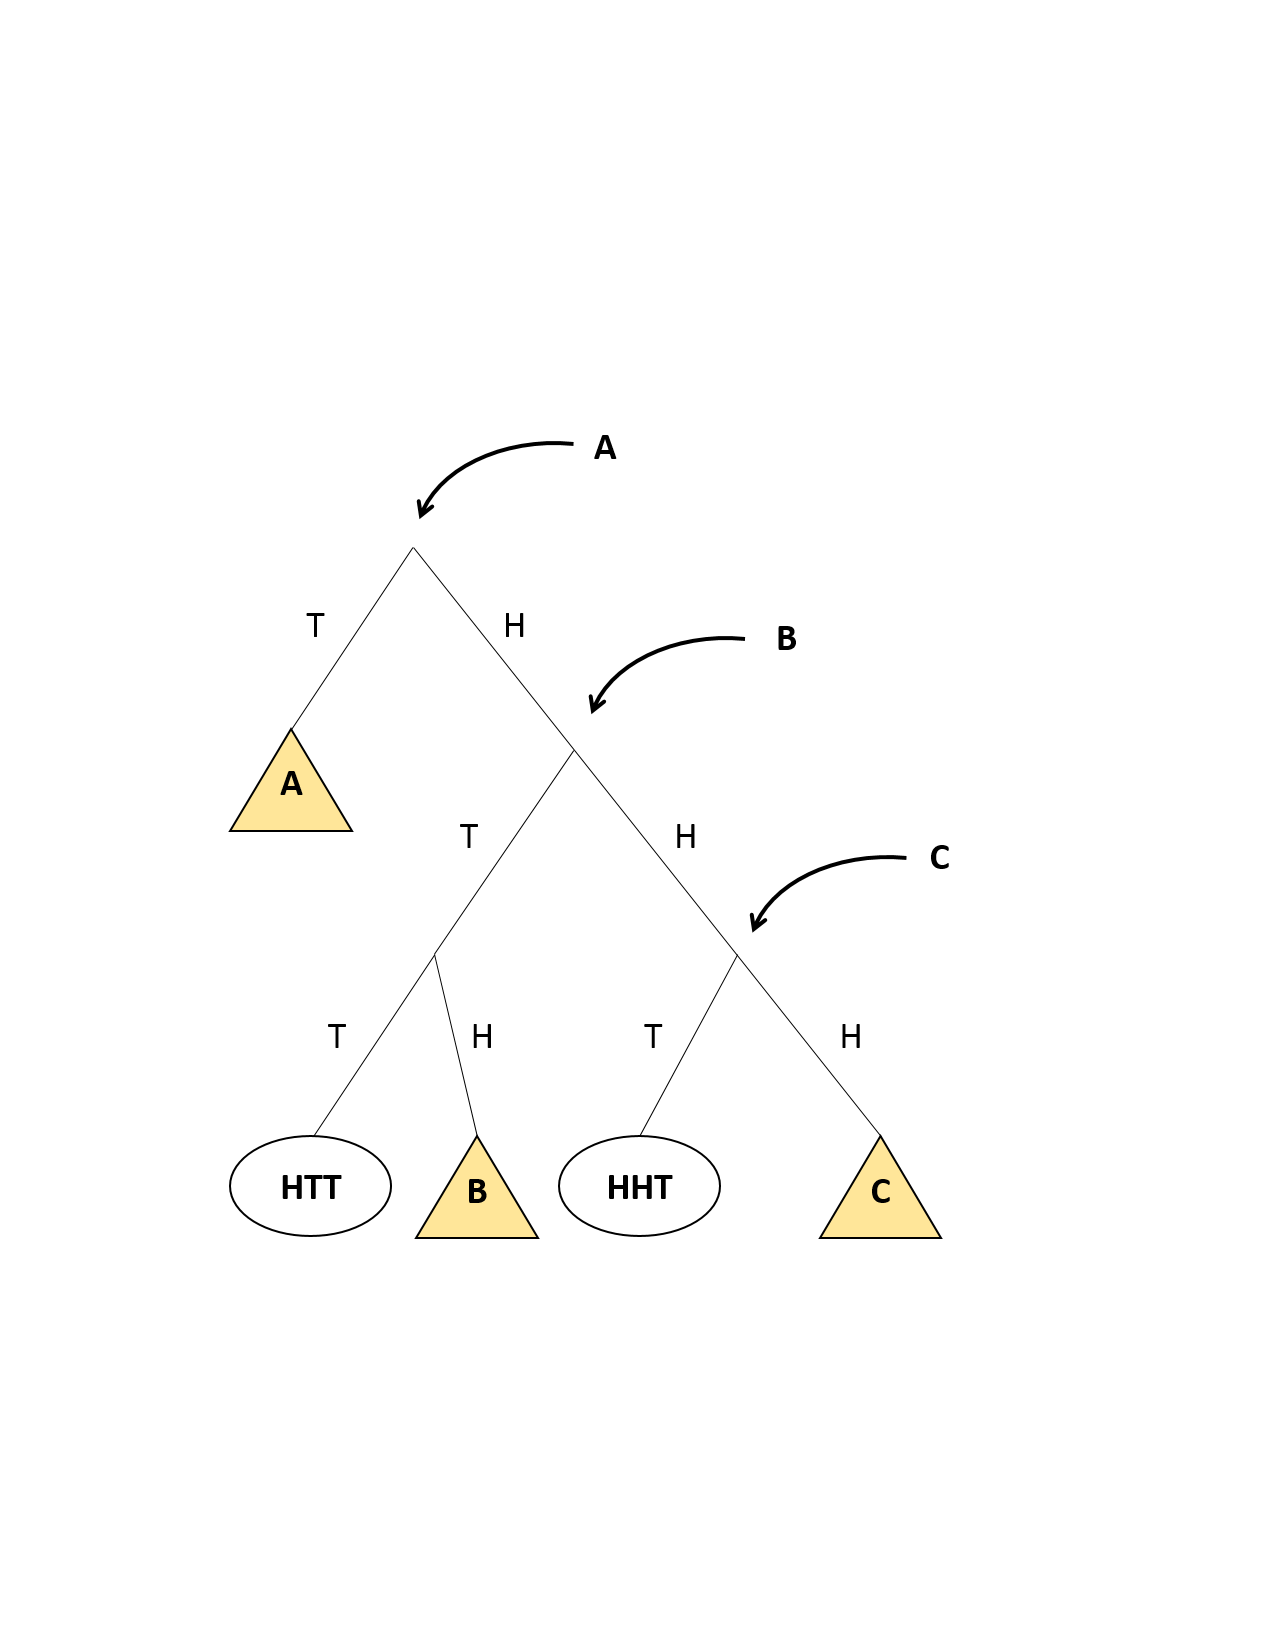
\includegraphics[width=4.5in]{HTT_HHT_race}
  \caption{STR{HTT} versus \STR{HHT}.}
  \label{HTTHHT}
\end{figure}

Summarizing we have:
\begin{align*}
\pr{A} &=
\prcond{A}{\tails}\pr{\tails}+\prcond{A}{\heads}\pr{\heads}
& \text{(Law of Total Probability)}\\
p & = p\frac{1}{2} + r\frac{1}{2} & \text{so}\\
p & = r.%\label{peq}
\end{align*}

Continuing, we have
\begin{align}
\prcond{A}{\heads}
&=
\prcond{A}{\mathtt{HT}}\pr{\tails}+\prcond{A}{\mathtt{HH}}\pr{\heads}
    & \text{(Law of Total Probability)}\notag\\
r &= \prcond{A}{\mathtt{HT}}\frac{1}{2} + 0\cdot\frac{1}{2}\label{here}\\
\prcond{A}{\mathtt{HT}} & =
\prcond{A}{\mathtt{HTT}}\pr{\tails}+\prcond{A}{\mathtt{HTH}}\pr{\heads}
& \text{(Law of Total Probability)}\notag\\
\prcond{A}{\mathtt{HT}} & = 1\cdot\frac{1}{2} + r\frac{1}{2} \label{there}\\
r & = (\frac{1}{2} + \frac{r}{2})\frac{1}{2} & \text{by~\eqref{here} \&~\eqref{there}}\notag\\
r & = \frac{1}{3}.\notag
\end{align}

So \STR{HTT} comes before \STR{HHT} with probability
\[
p=r =\cfrac{1}{3}.
\]

These kind of events have an amazing \idx{intransitivity} property: if
you pick \emph{any} pattern of three tosses such as \STR{HTT}, then
I can pick a pattern of three tosses such as \STR{HHT} whose odds
of coming up first are better then even.  If we then bet on which
pattern will appear first in a series of tosses, the odds will be in
my favor.  In particular, even if you instead picked the ``better''
pattern \STR{HHT}, there is another pattern I can pick that has a
more than even chance of appearing before \STR{HHT}.  So there are
cases where some pattern 1 appears before pattern 2 with probability
better than one half, and pattern 2 appears before some pattern 3 with
probability better than one half, but pattern 1 does \emph{not} appear
before pattern 3 with probability better than one half.

Watch out for this intransitivity phenomenon if somebody proposes that
you bet real money on coin flips.
\end{solution}

\end{problem}

%%%%%%%%%%%%%%%%%%%%%%%%%%%%%%%%%%%%%%%%%%%%%%%%%%%%%%%%%%%%%%%%%%%%%
% Problem ends here
%%%%%%%%%%%%%%%%%%%%%%%%%%%%%%%%%%%%%%%%%%%%%%%%%%%%%%%%%%%%%%%%%%%%%

\endinput
